
\documentclass[UTF8,12pt]{ctexart}



%二、字体
    %\setmainfont{fontName}  %英文的
    %\setsansfont{fontName}  %去设置-字体找fontName
    %\setmonofont{fontName}
    \setCJKmainfont{宋体}   %设置主字体族
    \setCJKsansfont{黑体}   %设置无衬线字体族
    \setCJKmonofont{楷体}   %设置打字机字体族
    %\textrm{}和\rmfamily, \textsf{}和\sffamily, \texttt{}和\ttfamily 
    %可以让我们分别主动调用主字体族,无衬线字体族和打字机字体族 

    %可以使用\textup{}和\upshape, \textit{}和\itshape
    %来分别主动调用当前字体族的直立体与意大利斜体

    %用\textmd{}和\mdseries, \textbf{}和\bfseries
    %来分别调用当前字体形状的正常体与粗体。



%字号:https://blog.csdn.net/c_arm/article/details/7013462



%五、行距与缩进
    \usepackage{setspace}  %行距
    \setstretch{1.2}       %填比例
    \setlength{\parskip}{1em}  %设置额外的段间距
    %  当前的字体大小被记作单位em, 也就是说,如果当前字号为12pt, 那当前1em=12pt.
    %  \setlength{\parindent}{2em}  设置缩进距离为2em
    %  \setlength{\parindent}{0em}  取消缩进



%六、附录与文献
    \newcommand{\upcite}[1]{\textsuperscript{\cite{#1}}} 
    %这使得我们可以在正文调用将编号置于右上角的参考文献

    \usepackage[toc, page]{appendix} 
    \renewcommand{\appendixtocname}{附录}
    \renewcommand{\appendixpagename}{附录}
    %这使得我们可以写附录



%七、列表
    \usepackage{enumitem}  %用于自定义列表

    %1. 定义问题一,问题二...列表,用question调用
        \newlist{question}{enumerate}{1}
        \setlist[question,1]{itemsep = 0pt, parsep = 0pt, align=left, leftmargin=*, label = {\bfseries 问题\chinese*}}

    %2. 定义问题一,问题二...列表,用zombie调用
        \newlist{zombie}{enumerate}{1}
        \setlist[zombie,1]{itemsep = 0pt, parsep = 0pt, align=left, leftmargin=*, label = {\bfseries 僵尸\chinese*}} 

    %\renewcommand{\theenumi}{\chinese{enumi}}
    %可以使第一级编号时出现的不是1 2 3而是一二三

    %\renewcommand{\labelenumi}{(\theenumi)}
    %可以使1.2.3.变成(1)(2)(3)

    %\renewcommand{\labelitemi}{随便符号}
    %可以改变无序列表的模样。比如填入空心圆圈$\circ$,或者更夸张填$\sum$等等



%八、纸张与页面
    \usepackage{fancyhdr}     %页面设置包
    \pagestyle{fancy}         
    \fancyhf{}
    \usepackage{geometry}  

    %1.页面与版心
        %(1)使用A4纸:               
        \geometry{a4paper}
        %(2)以数值形式指定纸张大小:   \geometry{paperheight=22cm, paperwidth=10cm}
        %(3)边距设置:边距有上下左右————left, right, top, bottom
            %\geometry{left=2cm}    %设置左边距为2cm
            %\geometry{right=2cm}
            %\geometry{top=2cm}
            %\geometry{bottom=2cm}
        %(4)版心水平居中:\geometry{hcentering}      版心竖直居中:\geometry{vcentering} 
        \geometry{hcentering}
        %(5)版心长设置:\geometry{textheight=20cm}   版心宽设置:\geometry{textwidth=20cm}

    %2.页眉与页脚    (先加载fancyhdr包)
        %(1)页眉页脚的左中右共6部分对应代码:
            %\lhead{}, \chead{}, \rhead{}, \lfoot{}, \cfoot{}, \rfoot{}
            \chead{“深圳杯”数学建模挑战赛}   
            \rhead{\thepage}
            %\chead{学习指南}  %在页眉正中出现“学习指南” 
        %(2)页眉线与页脚线:  \headrulewidth和\footrulewidth
            %\renewcommand\headrulewidth{0pt}   输入参数决定粗细,0则取消该线
            \renewcommand\headrulewidth{0pt}



%九、图片
    \usepackage{graphicx}           %四个包
    \usepackage{float}
    \usepackage{caption}
    \usepackage[export]{adjustbox}  %解决过宽图片

    %1.
    %\captionsetup[figure]{name=图片,font={Large, it}}   
    %将图片描述 “图X: ” 改成 “图片X: ”
    %将序号改为"it":意大利斜体,全部字体改成\Large
     
    %2.
    \captionsetup[figure]{name=图片} 
    %将图片描述设置为 “图片X: ”(默认)
    %texdoc caption 查看文档得到所有font,上面的it就是一种



%十、表格
    \usepackage{float}         %基础包
    \usepackage{booktabs}      %Excel2LaTeX美观选项支持
    \usepackage{longtable}     %过长表格
    %\usepackage{adjustbox}    %过宽表格包,但有另外的方法

    %1.
    \captionsetup[table]{font=large}
    %把“表 1”字体调大,格式类似九、2.



%十一、图片与表格的编号
    %\counterwithin{table}{section}    %让表格在section内编号
    %\counterwithin{figure}{section}   %让图片在section内编号
    %交叉引用!!!!:          使用\label \ref  均需要编译两次



%十二、数学
    \usepackage{amsmath}         %基础包
    \usepackage{esint}           %积分号美观包
    \usepackage{unicode-math}    %数学环境字体宏包

    %1.定义dx中d的立直体。用'\dif x'来输入正规的'dx'
    \def\dif{\mathop{}\!{}\mathrm{d}}




\begin{document}



\begin{titlepage}  %封面
    \centering
    \vspace*{\stretch{0}}{
        \huge{
            \textrm{
                2019\textbf{年“深圳杯”数学建模挑战赛}\\
                \ \\
                B\textbf{题}\\
                \ \\
                \ \\
                \ \\
                \textbf{新一代通信网络设计与规划}
            }
        }
    }\\

    \vspace{\stretch{2}}{
        \ \\
        \ \\
        \ \\
        \ \\
        \ \\
        \begin{align*}
            \text{\zihao{-2}中山大学:}\ \ &\text{\zihao{-2}林天皓}\\
            &\text{\zihao{-2}龙行健}\\
            &\text{\zihao{-2}卢浩文}
        \end{align*}
        }\\

    \vspace{\stretch{3}}
    {\today}
\end{titlepage}
    



%二、目录
\tableofcontents



%三、正文
\section{摘要}




\section{问题重述与分析}
    \subsection{微波问题}
    现有一个32单元相控天线阵列,移相器配置有4种方式$(0°,90°,180°,270°)$。
    采用仪器测量每种相位配置下的3D空间分布(数据参见附件一)。
    使用数据时需要考虑数据中存在的测量误差:移相器配置为$90°$和$180°$,
    两者信号相差$(90±err)°$,其中$err$为测量误差。
        \subsubsection{问题1}
            假设:\begin{enumerate}
                \item 合成功率为$35dBm$
                \item 旁瓣电平尽可能低
                \item 可以选择关闭某些通道
                \item 在位置$AZ=10°$,俯仰$EL=10°$处有一站点,
                    波束设计时避免对该站点的干扰
            \end{enumerate}
            请给出方位(水平角$AZ=10°$,俯仰角$EL=5°$)
            对应的波束配置(移相器配置矢量$\vec{z}=[∆_1,…,∆_N]$)
        \subsubsection{问题2}
            波束配置矢量要求:
                \begin{enumerate}
                    \item 整个覆盖区域内,平均辐射功率$35dBm$
                    \item 波束覆盖的“凹坑”尽可能小
                    \item 覆盖波束个数尽可能少
                    \item 用尽可能少的波束,覆盖水平角$±30°$,俯仰角$±15°$的区域
                \end{enumerate}
            请给出波束配置列表$[z_1,z_2,…,z_M]$(M为波束个数)
    \subsection{骨干网问题}
        随着众多网络接入技术的发展,以及未来用户数据需求量呈指数形式的增长,
        城市之间的骨干网输入输出端口带宽与容量需求也将爆炸式增长。
        使用最新的通信技术升级改造骨干网已成为运营商应对未来通信市场需求的一个迫在眉睫的举动。
        现需要在广东省对已有骨干网进行满足电信市场要求的改造。
        个人信息接入需求量会随着新科技在群众中的接受度,
        科技自身更迭速度等因素变化;同时各个年龄段,
        各收入阶层对信息需求量也有不同。
        \subsubsection{问题1}
            请预估未来十年(截止2028年)信息时代各类人群所需要的信息量,
            以满足广东省全部人口的信息接入需求为目标,省会广州市为数据中心,
            选择性地用最新的通信技术更新从广州到其余主要行政城市的骨干网络。
        \subsubsection{问题2}
            某通信公司曾提出:“建立一个万物互联的世界”。
            而在现实社会中,站在运营商角度,每个人的接入价值是不一样的,
            不同收入、地区、年龄的人接入成本和数据需求都不一样。
            如果将不同人群的网络接入价值也纳入考虑,
            并选择性的接入网络价值大的人群,请重新构建网络价值函数,
            并找到新的最优部署方案。
        



\section{模型假设}\label{mxjs}
    \subsection{微波问题}
    \subsection{骨干网问题}
        \begin{enumerate}
        \item 各个城市、人群的实际数据需求量总体随时间递增,但它并不是随时间一直增加的——
            例如,每一天,用户带宽需求都会随着时辰的改变而改变。
            信息网络的部署实际上应该着眼于每天/每周的用网高峰期。
            则在本文中,我们讨论的“数据需求量”均表示每天/每周用网高峰期的实际数据需求量。
        \item 如表格\ref{2g},从1991年2g网络诞生至今,我们熟知的移动网络通信标准大约10年更新一代。
        为了满足用户对信息容量与信息传输速度的需求,移动网络通信技术积极更新换代,
        其更新换代的速度大致可以反应所有网络通信技术更新换代的技术。
        假设在十年后广东省的总数据需求量已经达到了(所提供传输格式的)
        最大总容量$64Tb/s$的$90\%$,即$57.6Tb/s$。\\
        \Huge{此条为临时分析,等ldl的回归分析来取缔}\normalsize
        \begin{table}[htbp]
            \centering
              \begin{tabular}{ccccc}
              \toprule
              标准     & 2g     & 3g     & 4g     & 5g \\
              \midrule
              时间     & 1991   & 1998   & 2008   & 2020 \\
              \bottomrule
              \end{tabular}%              
            \caption{移动网络通信标准对应诞生时间}\label{2g}
          \end{table}%

        \item 骨干网承担各城市对外网络交互的出入口功能,起止点应该设于各个城市中心
            我们合理地假设所有光缆铺设的起止点位于各个城市的市政府附近,并以各市市政府
            位置为标准测量各城市间的距离。
            
        \item 光缆的铺设与维护是一项专业性工作,不需要像铺设公路考虑驾驶员安全一样苛刻。
            在铺设光缆时,只需要避开极端地形。不考虑海拔变化/地形因素对光缆长度的影响,
            我们合理地假设在两城间铺设光缆时,成本最低的方案大致为全线沿直线铺设。
        \end{enumerate}





\section{符号说明}
    \subsection{微波问题}
    \subsection{骨干网问题}





\section{模型建立}
    \subsection{微波相关1.2.3.4.5}


    \subsection{数据需求模型}\label{ShuJv}
            \begin{figure}[]
                    \centering
                    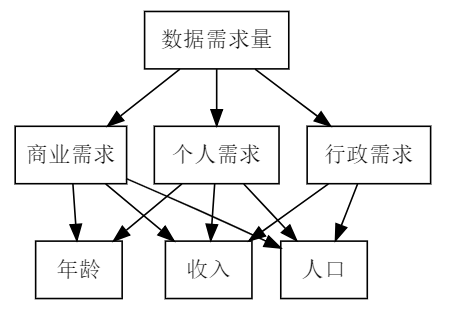
\includegraphics{need.png}
                    \caption{数据需求层次结构}\label{SJXQCCJG}
                \end{figure}
        建立层次结构模型,如图片\ref{SJXQCCJG}。                
        这三层分别为目标层O(数据需求量),准则层C,决定层D。

        \begin{enumerate}
            \item C层对数据需求量的影响:
            \begin{enumerate}
                \item 建立成对比较矩阵:
                $A_{C-O}=\begin{bmatrix}
                    1 & \frac{1}{4} & 4 \\                    
                    4 & 1 & 8\\                  
                    \frac{1}{4} & \frac{1}{8} & 1
                 \end{bmatrix}$
                \item 求得最大特征值$\lambda _{max}=3.0536$及其对应的权向量为
                    $$\overrightarrow\omega_{C-O}=(0.2227,0.7071,0.0702)$$
                \item 由$n_{c-o}=3$,求得$A_{C-O}$的一致性指标$CI_{C-O}=0.0268$
                \item 由$n_{c-o}=3$,得平均随机一致性指标$RI_{C-O}=0.58$,
                    则随机一致性比率$CR_{C-O}=0.0462<0.1$,接受该层分析。\\
            \end{enumerate}
            则认为商业需求,个人需求,行政需求对数据需求量影响的比重分别为$0.2227,0.7071,0.0702$。
              
            \item D层对数据需求量的影响:
            \begin{enumerate}
                \item 为D层对商业需求的影响建立成对比较矩阵:
                $$A_{D-C_1}=\begin{bmatrix}
                    1 & \frac{1}{8} & \frac{1}{6} \\
                    8 & 1 & 1\\
                    6 & 1 & 1
                 \end{bmatrix}$$
                \item 为D层对个人需求的影响建立成对比较矩阵:
                $$A_{D-C_2}=\begin{bmatrix}
                    1 & \frac{1}{2} & \frac{1}{8} \\
                    2 & 1 & \frac{1}{7}\\
                    8 & 7 & 1
                 \end{bmatrix}$$
                \item 为D层对行政需求的影响建立成对比较矩阵:\\(其中$D_1$不影响行政需求)
                $$A_{D-C_3}=\begin{bmatrix}
                    1 & \frac{1}{2}\\
                    2 & 1
                 \end{bmatrix}$$
                \item \begin{itemize}
                    \item 求得这三个成对比较矩阵的最大特征值向量为$$\lambda _{max}=(3.0092,3.0349,2)$$
                    \item 其对应的权向量矩阵为$$W_{D-C}=\begin{bmatrix}
                        0.0672 & 0.0813 & 0 \\
                        0.4887 & 0.1349 & 0.3333 \\
                        0.444  & 0.7838 & 0.6667
                     \end{bmatrix}$$
                    \item 对应的D层对O层的组合权向量为$$\omega_{D-O}=\begin{bmatrix}
                        0.0672 & 0.0813 & 0 \\
                        0.4887 & 0.1349 & 0.3333 \\
                        0.444  & 0.7838 & 0.6667
                     \end{bmatrix}×\begin{bmatrix}
                        0.2227 \\
                        0.7071 \\
                        0.0702
                     \end{bmatrix}=\begin{bmatrix}
                        0.0725 \\
                        0.2276 \\
                        0.6999
                     \end{bmatrix}$$
                    \end{itemize}                    
                \item 则D层对C层的一致性指标为
                    $$CI_{D-C}=[0.0046,0.0174,0]×\begin{bmatrix}
                    0.2227 \\
                    0.7071 \\
                    0.0702
                     \end{bmatrix}=0.0133$$
                \item 又有D层对C层的平均随机一致性指标为
                    $$RI_{D-C}=[0.58,0.58,0]×\begin{bmatrix}
                    0.2227 \\
                    0.7071 \\
                    0.0702
                     \end{bmatrix}=0.5393$$
                \item 则D层对O层的组合随机一致性比率为
                    $CR_{D-O}=0.0462+\displaystyle\frac{0.0133}{0.5393}=
                    0.0709<0.1$,接受该层分析。
            \end{enumerate}

        \end{enumerate}
        综上,得到年龄,收入,人口对数据需求量影响的比重分别为$0.0725,0.2276,0.6999$
        


    \subsection{城市评分模型}\label{PingFen}
        \subsubsection{平均年龄评分}
            当今社会中的年轻人,特别是大学生使用互联网教多,数据需求量较大。
            数据需求量的峰值大约在年龄为15岁~25岁之间达到。
            广东省内各城市平均年龄均大于30岁,则年龄与数据需求量大致可视为负相关,
            则选择以反比例尺度对平均年龄评分
            \begin{itemize}
                \item 以广州市的平均年龄$Y_0=34.4$岁为100分
                \item 某市$C_k$的平均年龄为$Y_k$,满足$Y_0=\displaystyle\frac{x_{k2}}{100}·Y_k$,则该市年龄得分为$x_{k2}$
                \item 任一城市$C_k$的年龄得分为$$x_{k2}=\frac{100Y_0}{Y_k}$$
            \end{itemize}

        \subsubsection{人均可支配收入评分}
            数据需求量应当与收入呈正相关,但随着收入的增加,
            数据需求量的增长率不会一直保持水平,应该随收入的增加而逐渐降低。
            则选择以对数尺度对人均可支配收入评分:
            \begin{itemize}
                \item 以广州市人均可支配收入为100分\par 
                    (\ 设广州市人均可支配收入$I_0=5.5356=a^{100}$万元\ )
                \item 某市$C_k$的人均可支配收入$I_k=a^{x_{k1}}$万元,则该市收入得分为$x_{k1}$
                \item 任一城市$C_k$的收入得分为$$x_{k1}=\log _{I_0}({I_k}^{100})=\frac{100\ln I_k}{\ln I_0}$$
            \end{itemize}

        \subsubsection{人口评分}
            由于城市需求量大致是每个群体的群体需求量的总和,
            所以人口与数据需求量大致成线性关系。则选择以线性尺度对城市人口评分
            \begin{itemize}
                \item 以广州市的人口$P_0=1490.44$万人为100分
                \item 某市$C_k$的人口为$P_k$,则该市的人口得分为$$x_{k3}=\frac{100P_k}{P_0}$$
            \end{itemize}
 




\section{问题求解}
    \subsection{微波问题1}
    \subsection{微波问题2}
    \subsection{骨干网问题1}
        \subsubsection[网络需求评估]{网络需求评估}
            对广东省各城市人口、平均年龄、人均可支配收入\upcite{SJ},
            根据\ref{PingFen}城市评分模型进行评分,
            并根据\ref{ShuJv}数据需求模型评价各个城市的需求总分。
            以xxxxxxx为标准,得到单位分数对应的数据需求量,
            以此评估广东省各城市的数据需求量。            
    \subsection{骨干网问题2}



%四、附录
\begin{appendices}
    \addtocontents{toc}{\protect\setcounter{tocdepth}{0}}
    \section{第一个}
        可以再使用subsection
    \section{第二个}
        同上
    %可以看到这些section不会出现在目录里头,而只有“附录”一个代表。
    \end{appendices} 



%五、文献
\begin{thebibliography}{20}   %表示参考文献最大数量
    %每个bibitem表示一份文献
    %第一个参数这里没用(不显示),用于交叉引用
    %第二个参数就是显示的内容
    \bibitem{Lxh}{李相赫,《教你玩中单》,召唤师峡谷:峡谷出版社, 2015.}
    \bibitem{RR}{金泰相,论中路混子的基本素养,洲际赛日报,2018,S(8):02-03,2018.}
    \bibitem{sm}{王思聪,论我为何没有马,http://www.wscnomom.cnm,2018.11.11.}
    \bibitem{SJ}{广东省统计局,广东统计信息网(及首页中各市链接), http://stats.gd.gov.cn/, 2019.5.12.}
\end{thebibliography}

\end{document}
            